\chapter{Digital filtering}\label{ch:filter}

A filter keeps some frequencies and suppresses others. The application offers a band-pass filter on the Data,
Live and Helicorder pages: slow drifts below the lower corner and electrical or traffic noise above the upper
corner are removed, leaving the band in which the phenomenon of interest lives.

\section{Frequency response of a digital filter}
A linear filter acts on a sampled signal by convolution, $y[n]=\sum_m h[m]\,x[n-m]$. Its effect at frequency $f$ is
described by $H(f)=\sum_m h[m]\,e^{-\jj 2\pi f m/\fs}$, a complex number whose magnitude is the \emph{gain} and whose
angle is the \emph{phase shift}. A band-pass filter has gain close to 1 between two \emph{corner frequencies}
$f_1<f_2$ and gain close to 0 outside.

\section{The Butterworth filter}
Among the classical filter families, the Butterworth filter \parencite{butterworth1930} has the property that its
magnitude is as flat as possible in the pass band. The magnitude of a Butterworth low-pass filter of order $n$ and
cut-off $\omega_c$ is
\begin{equation}\label{eq:butter}
  \abs{H(\jj\omega)}^{2} = \frac{1}{1+\left(\omega/\omega_c\right)^{2n}} .
\end{equation}
At $\omega=\omega_c$ the gain is $1/\sqrt2$, that is $-3$~dB, for every order. Beyond the cut-off the gain falls by
$20n$~dB per decade ($6n$~dB per octave), so a higher order gives a steeper edge. A band-pass filter is obtained from a
low-pass prototype by the substitution $s\mapsto (s^{2}+\omega_1\omega_2)/\bigl(s(\omega_2-\omega_1)\bigr)$, which
doubles the number of poles: an order-$n$ band-pass has $2n$ poles. Digital implementations realise the filter as a
cascade of second-order sections (SOS) rather than one high-order polynomial, because the cascade is numerically
far more stable.

\begin{figure}[tbp]
\centering
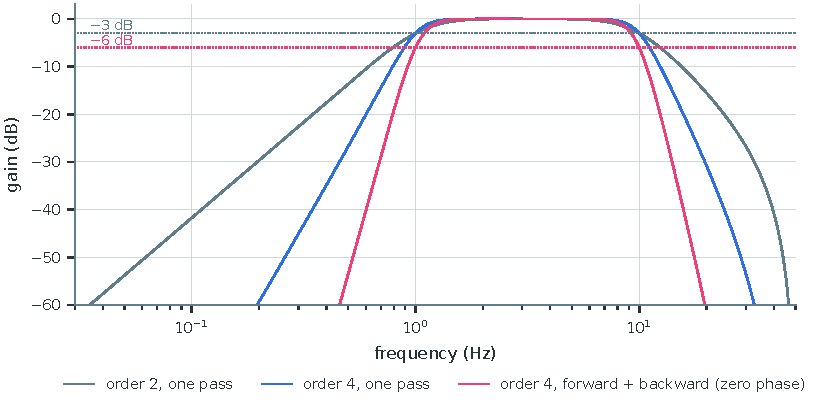
\includegraphics[width=\linewidth]{theory-butterworth}
\caption{Gain of band-pass Butterworth filters with corners 1 and 10~Hz at $\fs=100$~Hz: order~2 and order~4 in a
single pass, and order~4 applied forward and backward (zero phase), whose gain in decibels is exactly twice that of
one pass.}\label{fig:butter}
\end{figure}

\section{Zero-phase filtering}
A causal filter delays different frequencies by different amounts (phase distortion), which smears and shifts
waveforms. A standard remedy is to filter the record forward, reverse the output, filter it again, and reverse the
result. If one pass has frequency response $H(f)$, the backward pass contributes $H^{*}(f)$ (the complex conjugate),
so the combined response is
\begin{equation}\label{eq:zerophase}
  H_{\mathrm{zp}}(f) = H(f)\,H^{*}(f) = \abs{H(f)}^{2},
\end{equation}
a real, non-negative number: \emph{zero phase shift}. Two consequences follow from~\eqref{eq:zerophase}:

\begin{enumerate}
\item \textbf{The gain in decibels doubles.} The $-3$~dB corner of a single pass becomes a $-6$~dB corner
  (\cref{fig:butter}), and the roll-off steepens to $12n$~dB per octave.
\item \textbf{The filter is non-causal.} The output at time $t$ depends on input after $t$.
\end{enumerate}

\begin{rs3dwarn}[Non-causal filters move energy before the onset]
A zero-phase filter smears the sharp start of an arrival \emph{backwards} in time, as \cref{fig:zerophase} shows: the
filtered record contains oscillations before the true onset. Zero-phase filtering is therefore appropriate for
looking at a waveform, but it must not be used to pick onset times or to drive a real-time trigger. The detector of
Chapter~\ref{ch:detect} uses a causal filter for exactly this reason.
\end{rs3dwarn}

\begin{figure}[tbp]
\centering
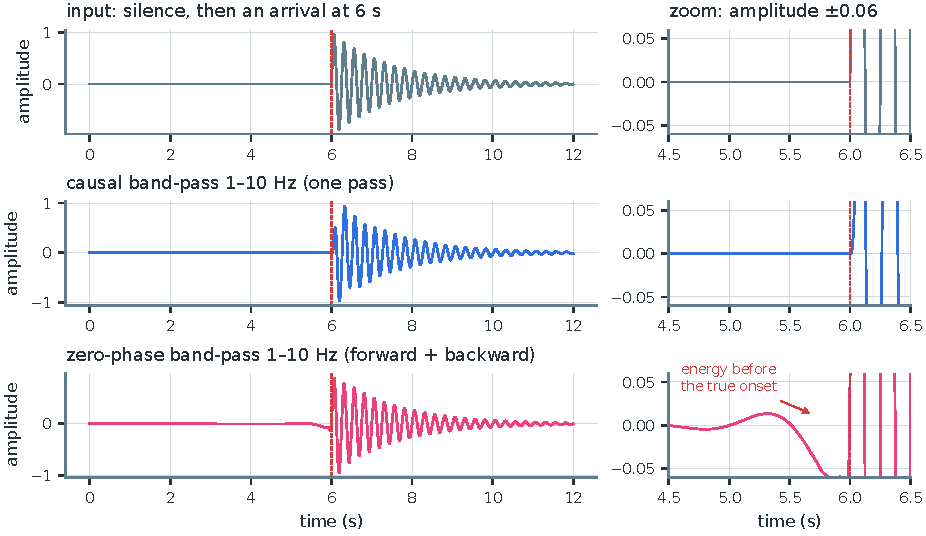
\includegraphics[width=\linewidth]{theory-zerophase}
\caption{An ideal arrival at 6~s filtered by a 1--10~Hz band-pass, causally (one pass) and with zero phase. The
causal output is exactly zero before the arrival; the zero-phase output rings before it (enlarged on the right).
The zero-phase curve was computed with SciPy's padded \code{sosfiltfilt}.}\label{fig:zerophase}
\end{figure}

\section{Edge effects}
A filter has a memory: its output near the start of a record depends on samples that were never recorded. The first
and last seconds of a filtered trace contain a \emph{transient} and are less reliable. The effect is largest for narrow
bands and low corners; a practical rule is to distrust about $3/f_1$ seconds at each end. The same holds at
every \emph{gap}: each contiguous piece of a trace is filtered on its own, so the edges of each piece carry a
transient.

\section{Choosing a band}
\Cref{tab:bands} lists bands commonly used with a short-period sensor such as the RS3D. They are starting points, not
rules; the right band depends on the noise at the site (Chapter~\ref{ch:noise}).

\begin{table}[tbp]
\centering\small
\caption{Typical pass bands for three-component short-period data.}\label{tab:bands}
\begin{tabularx}{\linewidth}{@{}l c X@{}}
\toprule
Purpose & Band (Hz) & Comment\\ \midrule
Local and regional earthquakes & 1--10 & the RS3D live default; rejects drift and most wind or traffic noise\\
Teleseismic body waves & 0.5--3 & the Shake's sensitivity falls quickly below its 4.5~Hz natural frequency\\
Microseism & 0.1--0.5 & strong everywhere; useful as a check of the instrument\\
Cultural noise & 5--25 & footsteps, traffic, machinery\\
\bottomrule
\end{tabularx}
\end{table}

\begin{rs3dapp}
RS3D uses two different implementations, deliberately.
\begin{itemize}
\item \textbf{Data and Helicorder pages, exports} (\file{core/export.py}). ObsPy's
  \code{filter("bandpass", freqmin, freqmax, corners=4, zerophase=True)} after \code{detrend("demean")}.
  Reading the library source and comparing outputs shows that ObsPy implements \code{zerophase} as two passes of an
  SOS filter (forward, then backward) \emph{without} padding, so edge transients are visible; the result is identical
  to two calls of \code{sosfilt}. Corner~4 means a 4th-order design, so the effective roll-off is 48~dB per octave per
  edge.
\item \textbf{Live page} (\file{core/live.py}). SciPy's \code{butter(2, [f\_min, min(f\_max, 0.45 fs)])} applied with the
  padded \code{sosfiltfilt} to each contiguous chunk of the ring buffer, after removing the chunk's mean. The upper
  corner is limited to $0.45\,\fs=45$~Hz to stay below the Nyquist frequency, and a chunk shorter than the padding
  length is only demeaned and not filtered.
\end{itemize}
Both give a zero-phase band-pass; they differ in order and in edge treatment. The numbers a filtered Live trace shows
therefore differ slightly from the same interval exported from the Data page.
\end{rs3dapp}

\section{Summary}
\begin{rs3dkey}
A Butterworth band-pass applied forward and backward is a zero-phase filter whose corner gain is $-6$~dB, whose
roll-off is twice that of one pass, and which is \emph{not} causal. Use it to look at waveforms; use a causal filter
to detect them.
\end{rs3dkey}
